\documentclass[a4paper,11pt,twoside]{article}

\usepackage{palatino,newtxmath,bbold}	%% Písma
\usepackage{microtype}					%% Lepší mezery
\usepackage[T1]{fontenc}
\usepackage[utf8]{inputenc}	            %% Kódování textu
\usepackage{amsfonts,amsmath}			%% Matematické symboly (amssymb koliduje s jiným balíkem)

\usepackage{epsfig}                     %% Obrázky
\usepackage[subrefformat=simple,labelformat=simple]{subcaption} %% Podobrázky
\usepackage{graphicx}					%% Doplňující příkazy pro obrázky

\usepackage{xifthen}					%% Podmínka if - then
\usepackage{makeidx}					%% Rejstřík
%\usepackage{showframe}
%\usepackage{showidx}

\usepackage[multiple]{footmisc}			%% Lepší formátování poznámek pod čarou - nefunguje s hyperref
%\usepackage{fnpct}						%% Lepší formátování poznámek pod čarou
\usepackage{comment}					%% Komentáře
\usepackage{scrextend}					%% Vylepšené formátování (addmargin)
\usepackage{xcolor}						%% Barvy
\usepackage{indentfirst}				%% Odsazení prvního odstavce
\usepackage{fancyhdr}
\usepackage{blkarray}					%% Pro komentované vektory
\usepackage{empheq}                     %% Box around equations

\usepackage{csquotes}
\usepackage{expl3}						%% Jinak nefunguje biblatex
\usepackage{biblatex}
\addbibresource{S:/Fyzika/Bibliography/References.bib}

%\bibliographystyle{phaip}

\graphicspath{{figures/}}

%\usepackage{showlabels}                 %% Temporarily show the names of labels
%\renewcommand{\showlabelfont}{\tiny\bfseries\color{black}}

\usepackage{mathtools}
%\mathtoolsset{showonlyrefs}            %% Remove equation number of unrefferenced equations

\usepackage[unicode]{hyperref}			%% Hypertextové odkazy
\hypersetup{
	pdftitle={Notes on Rabi's cat},
	pdfauthor={Das Pavel},
	pdffitwindow=true,
	colorlinks=true,
	urlcolor=cyan,            			%barva textu pri tisku
	linkcolor=red,
	citecolor=green,
	filecolor=magenta
}

% Velikost stránky
\addtolength{\topmargin}{-1.5cm} %\addtolength{\textheight}{-10cm}
\addtolength{\textwidth}{4cm} \addtolength{\textheight}{4cm} % Šířka a výška textu
\addtolength{\voffset}{-0.5cm} % Horní okraj
\addtolength{\hoffset}{-2cm}
\setlength{\headheight}{15pt}

\pagestyle{fancy}

% Definice
\DeclareMathOperator{\e}{e}
\DeclareMathOperator{\tg}{tg}
\DeclareMathOperator{\cotg}{cotg}
\DeclareMathOperator{\arccotg}{arccotg}
\DeclareMathOperator{\sign}{sign}
\DeclareMathOperator{\arccosh}{arccosh}
\DeclareMathOperator{\arcsinh}{arcsinh}
\DeclareMathOperator{\divergence}{div}
\DeclareMathOperator{\gradient}{grad}
\DeclareMathOperator{\trace}{Tr}
\DeclareMathOperator{\real}{Re}
\DeclareMathOperator{\imaginary}{Im}
\DeclareMathOperator{\Ai}{Ai}
\DeclareMathOperator{\Bi}{Bi}
\DeclareMathOperator{\Tp}{\mathsf{T}}

\renewcommand{\d}{\mathrm{d}}
\newcommand{\D}{\mathcal{D}}

\def\O#1{\mathcal{O}\left({#1}\right)}

\def\ket#1{\left|{#1}\right\rangle}
\def\bra#1{\left\langle{#1}\right|}
\def\mean#1{\left\langle{#1}\right\rangle}
\def\braket#1#2{\left\langle{#1}\middle|{#2}\right\rangle}
\def\matrixelement#1#2#3{\left\langle{#1}\middle|{#2}\middle|{#3}\right\rangle}
\def\ketbra#1#2{\left|{#1}\middle\rangle\middle\langle{#2}\right|}
\def\projector#1{\left|{#1}\middle\rangle\middle\langle{#1}\right|}

\def\unit#1{\,\mathrm{{#1}}}
\def\c{,\!}

\def\hi#1{^{({#1})}}

\def\clebsch#1#2#3#4#5#6{\mathcal{C}^{#5\,#6}_{#1\,#2\:#3\,#4}}
\def\threej#1#2#3#4#5#6{\begin{pmatrix}#1&#2&#3\\#4&#5&#6\end{pmatrix}}

\def\commutator#1#2{\left[{#1},{#2}\right]}
\def\associator#1#2#3{\left[{#1},{#2},{#3}\right]}

\def\abs#1{\left|{#1}\right|}
\def\abss#1{\left|{#1}\right|^{2}}							% Square of the absolute value
\def\intinf{\int_{-\infty}^{\infty}}						% Infinite integral

\def\minus#1{\left(-1\right)^{#1}}
%\def\ui#1{(#1)}
\def\ti#1{\mathrm{#1}}										% Text index

\def\error#1{{\color{red}{\bf{#1}}}}
\def\trick#1{{\color{blue}#1}}

\def\hilbert#1{\mathcal{#1}}								% Hilbert space
\def\group#1{\mathrm{#1}}									% Group
\def\algebra#1{\mathrm{#1}}

\def\vector#1{\boldsymbol{#1}}								% Vector
\def\matrix#1{\mathsf{#1}}										% Matrix
\def\axis#1{\mathrm{#1}}

\def\2F1#1#2#3#4{\,{}_{2}F_{1}\!\left(#1,#2,#3;#4\right)}
\def\1F1#1#2#3{\,{}_{1}F_{1}\!\left(#1,#2;#3\right)}

\def\operator#1{\mathsf{\hat{#1}}}
\def\vectoroperator#1{\boldsymbol{\mathsf{\hat{#1}}}}
\def\tensoroperator#1#2{\hat{\mathbb{#1}}^{(#2)}}					% tensor operator
\def\tensoroperatorcomponent#1#2#3{\hat{\mathsf{#1}}^{(#2)}_{#3}}	% tensor operator - component
\def\reducedmatrixelement#1#2#3{\left(#1\middle\lVert#2\middle\rVert#3\right)}	    % Reduced matrix element

\def\propagator{G(\vx_{\rf},t_{\rf};\vx_{\ri},t_{\ri})}

\newcommand{\partialderivative}[3][]{\ifthenelse{\isempty{#1}}	% Partial derivative
	{\frac{\partial{#2}}{\partial{#3}}}
	{\frac{\partial^{#1}{#2}}{\partial{#3}^{#1}}}
}

\newcommand{\derivative}[3][]{\ifthenelse{\isempty{#1}}	% Normal derivative
	{\frac{\d{#2}}{\d{#3}}}
	{\frac{\d^{#1}{#2}}{\d{#3}^{#1}}}
}

\def\conjugate#1{{#1}^{\dagger}}
\def\transpose#1{{#1}^{\intercal}}

\def\operatorconjugate#1{\conjugate{\operator{#1}}}

\def\makematrix#1{\begin{pmatrix}#1\end{pmatrix}}       % Matrix
\def\Vdots{\vphantom{0}\smash[t]{\vdots}}

\def\equationcomment#1{\begin{vmatrix}#1\end{vmatrix}}  % Comment in equation (e.g. substitution in integral)

\long\def\important#1{\boxed{#1}}

\def\MeV{\mathrm{MeV}}
\def\im{\mathrm{i}}
\def\const{\mathrm{const}}

\includecomment{theory}
%\excludecomment{solution}
%\includecomment{note}

% Homework - části, které jsou (byly) za domácí úkol, a proto by se neměly vyskytnout ve sbírce
%\excludecomment{homework}

% homeworknote - části, které jsou navázané na řešení; část s domácím úkolem; vzájemně exklusivní s prostředním homework
\newenvironment{homeworknote}{}{}

% Toto se odkomentuje pro tištěnou kompletní sbírku
%\excludecomment{homeworknote}
\newenvironment{homework}{}{}

% solution - část s řešením
%\excludecomment{solution}
%\excludecomment{theory}
\newenvironment{solution}{\begin{addmargin}{0.5cm}\color{gray}\subsubsection*{Řešení:}\small}{\end{addmargin}\vspace*{0.3cm}}

\newenvironment{example}{\textbf{\textit{Příklad:}}}{}

\newenvironment{note}[1][]{\vspace*{0.2cm}\noindent\textbf{\textit{\ifthenelse{\isempty{#1}}{Poznámka: }{#1}}}}{}
%\newenvironment{theory}{}{}

\def\sec#1{\subsubsection*{#1}}
\def\sfootnote#1{\footnote{\color{gray}#1}}
\def\scaption#1{\caption{\small\color{gray}#1}}
\def\scaptionx#1#2{\caption[#1]{\small\color{gray}#2}}

\newcommand{\np}{\clearpage\newpage}
%\newcommand{\np}{\clearpage\setcounter{page}{1}\newpage}
%\newcommand{\np}{}\newcommand{\minput}[1]{\input{#1}}

\newcommand{\exercise}[2][]{\ifthenelse{\isempty{#1}}
	{\np\thispagestyle{empty}\subsubsection*{Domácí úkol -- #2}}
	{\np\thispagestyle{empty}\np\subsubsection*{Domácí úkol -- #2 \small{\it{(termín odevzdání: {#1})}}}}
}

\makeindex

\begin{document}

\title{Notes on the Rabi's Cat}
\date{\today}
\author{Das Pavel}

\maketitle
\section{Model}
	Parity violating Rabi model
	\begin{equation}
		\label{eq:H}
		\operator{H}=
			\omega\operatorconjugate{b}\operator{b}+\omega R\left(\operator{J}_{z}+j\right)
			+2\sqrt{R}\lambda\left[\left(\operatorconjugate{b}+\operator{b}\right)\operator{J}_{z}-\im\delta\left(\operatorconjugate{b}-\operatorconjugate{b}\right)\operator{J}_{y}\right]
			+\mu\left(\operatorconjugate{b}+\operator{b}\right)\left(\operator{J}_{z}+j\right),
	\end{equation}
	\begin{itemize}
		\item
			$\vectoroperator{J}=\left(\operator{J}_{x},\operator{J}_{y},\operator{J}_{z}\right)$ is the quasispin (qubit) operator with size $j=1/2$.

		\item 
			$\operator{b},\operatorconjugate{b}$ are the field (oscillator) annihilation and creation operators.

		\item 
			$\omega$ is the field frequency.

		\item
			$R\gg1$ is the detunning between the quasispin and the oscillator, and plays the role of the size parameter of the system.

		\item 
			$\lambda$ is the quasispin-field interaction strength. 

		\item
			$\delta$ interpolates between the ($\delta=1$) Jaynes-Cummings regime, ($\delta=0$) Rabi regime and ($\delta=-1$) anti-Jaynes-Cummings regime.

		\item
			$\mu$ governs the strength of parity-violation.
	\end{itemize}

\section{Critical structure}
	We focus on the excited-state quantum phase transition (ESQPT) at $E=0$.
	Its character is given by the index $k$ of the corresponding nondegenerate stationary point in the infinite-$R$ limit of the Hamiltonian~\eqref{eq:H}, and it changes with increasing interaction strength $\lambda$ at two critical points
	\begin{align}
		\lambda_{c}&=\frac{\omega}{2},\\
		\lambda_{0}&=\frac{\lambda_{c}}{\abs{\delta}}.
	\end{align}
	\begin{itemize}
		\item $\lambda<\lambda_{c}$ (normal phase, N): $k=0$, stable dynamics,
		\item $\lambda_{c}<\lambda<\lambda_{0}$ (superradiant phase I, S1): $k=1$, unstable dynamics,
		\item $\lambda>\lambda_{0}$ (superradiant phase II, S2): $k=2$, stable dynamics.
	\end{itemize}

\section{Numerical study}
	In the calculations, the following values of the parameters are taken:
	\begin{equation}
		\omega=1,\qquad
		\delta=\frac{1}{2},\qquad
		\lambda=\frac{3}{4},\qquad
	\end{equation}
	so the system is situated in the middle of phase S1.
	We evolve the initially factorized state $\ket{\psi(0)}=\ket{-\frac{1}{2}}\otimes\ket{0}$ (both quasispin and field are in their lowest state) and calulate expectation values $\matrixelement{\psi(t)}{\bullet}{\psi(t)}$ of the following operators:
	\begin{itemize}
		\item $J_{x}$ (first component of the quasispin operator),
		\item $\operator{q}=\frac{1}{2\sqrt{jR}}\left(\operatorconjugate{b}+\operator{b}\right)$ (coordinate).
	\end{itemize}
	The expectation value of both operators vanishes at all times if the parity is conserved $\mu=0$.

\section{Results}
The numerical results for the expectation values of operators $\operator{q}, \operator{J}_{x}$ sensitive to the parity violation are displayed in Figures~\ref{fig:q}---\ref{fig:fullqJx}.
Note that similar behaviour is observed for operators $\operator{p}, \operator{J}_{y}$.
The product $\mu R$ is kept constant, which makes the curves roughly coincide with one another.
The value of this product is chosen so that the first significant minimum of $q(t)$ is the deepest.

Scalling $t'=st$ in Figures~\ref{fig:q} and~\ref{fig:Jx} makes the first pronounced minimum of $q$ at $t_{\mathrm{min}}\approx13R^{0.1}$ sit approximately at the same time $t'$.

The first small dip, observed in Figure~\ref{fig:q}~(b) at $t'\approx7$ is caused by different depths of the left and right well. 
This difference is getting smaller with decreasing $\mu$, and in the limit $R\rightarrow\infty$, $\mu R=\const$ vanishes.
On the other hand, the well-pronounced minimum at $t'\approx20$ is caused by the phase difference between the orbits in the left and right well, and its magnitude doesn't change with $\mu$, provided the product $\mu R$ is kept constant.
The same is observed for the first derivative $q'(t)$ in Figure~\ref{fig:qd}.

Figure~\ref{fig:fullqJx} shows that the first important extreme of $q(t)$ and $J_{x}(t)$ occurs for a fixed $R$ approximately at the same time $t$.
There exists the smallest $\mu_0$ for which the phenomenon is present (the centre of the leftmost lowest blue region in the second panel), and then there is a sequence of alternating minima-maxima both in $q$ and $J_{x}$ at $\mu=k\mu_{0}$, $k=1,2,3,4,\dotsc.$.
This is related to the difference of phases between wavepackets in both wells.

\begin{figure}[!h]
        \begin{subfigure}{0.49\linewidth}
            \centering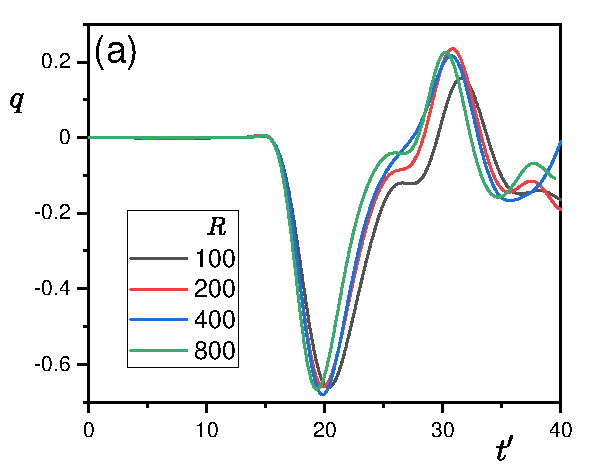
\epsfig{file=q.pdf,width=\linewidth}
        \end{subfigure}
        \hfill
        \begin{subfigure}{0.49\linewidth}
            \centering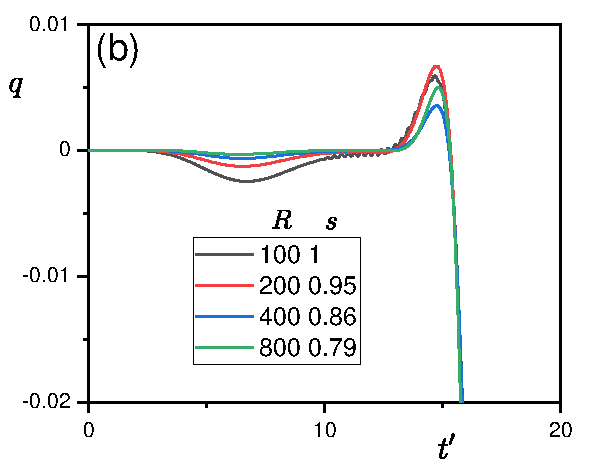
\epsfig{file=qdetail.pdf,width=\linewidth}
        \end{subfigure}
		\caption{Expectation value $q(t)=\matrixelement{\psi(t)}{\operator{q}}{\psi(t)}$ for different system sizes $R$ and for a perturbative value of $\mu$ reciprocal to the system size $\mu=0.13/R$.
		The magnitude of the parity violation is observed to be independent of the system size. (a) Full image. (b) Detail to the pre-parity-violation. 
		Note that in both panels the time is rescalled via $t'=st$ and $s$ is indicated in the legend of panel (b).}
		\label{fig:q}
	\end{figure}   	

	\begin{figure}[!h]
        \begin{subfigure}{0.49\linewidth}
            \centering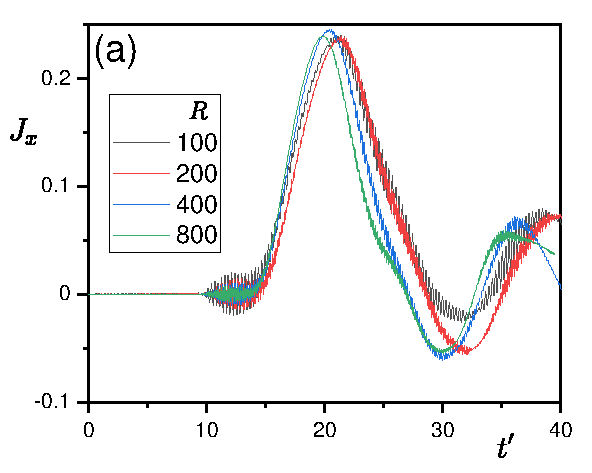
\epsfig{file=Jx.pdf,width=\linewidth}
        \end{subfigure}
        \hfill
        \begin{subfigure}{0.49\linewidth}
            \centering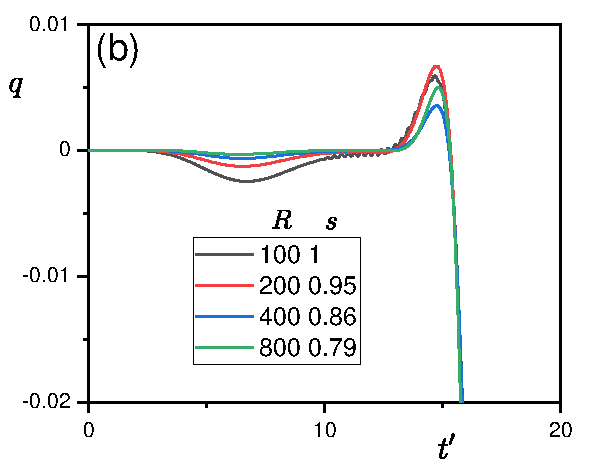
\epsfig{file=qdetail.pdf,width=\linewidth}
        \end{subfigure}
		\caption{The same as in Figure~\ref{fig:q}, but here for expectation value $J_{x}(t)=\matrixelement{\psi(t)}{\operator{J}_{x}}{\psi(t)}$.
		Note the fast oscillations caused by the detuning given by $R$.}
		\label{fig:Jx}
	\end{figure}   	

	\begin{figure}[!h]
        \centering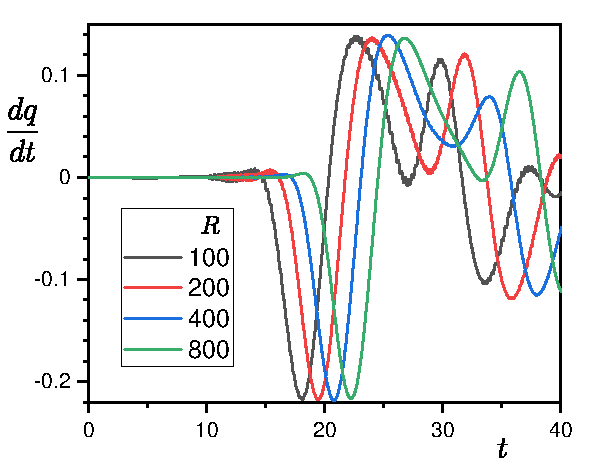
\epsfig{file=qd.pdf,width=0.5\linewidth}
		\caption{The first derivative of $q(t)$.}
		\label{fig:qd}
	\end{figure}   	

	\begin{figure}[!h]
        \centering\epsfig{file=jx q 200.0.png,width=\linewidth}
		\caption{Full image of $J_{x}$ and $q$ as a function of $t$ (vertical axis) and $\log_{10}\mu$ (horizontal axis) for $R=200$.}
		\label{fig:fullqJx}
	\end{figure}   	

%\bibliography{Z:/Share/Fyzika/Bibliography/References.bib}
\printbibliography
%\input{refs}

\end{document}

